% !TEX program = xelatex

\documentclass{resume}
\usepackage{graphicx}
\usepackage{tabu}
\usepackage{multirow}
\usepackage{ctex}
\usepackage{color}
\usepackage{progressbar}
\usepackage{hyperref}


\begin{document}

\begin{center} 
\Large\textbf{明廷来个人简历}
\end{center}
\pagenumbering{gobble} % suppress displaying page number

{
% change Large font here
\Large{
  \begin{tabu}{ c l }
   \multirow{5}{1in}{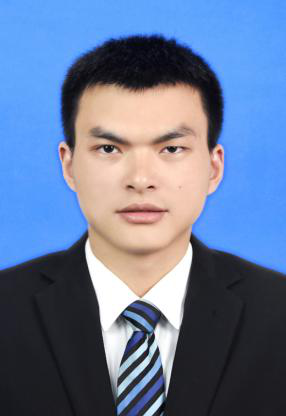
\includegraphics[width=0.88in]{mingtinglai}} & \scshape{MingTinglai} \\ 
    &\email{tlming16@fudan.edu.cn} \\ 
    &\phone{(+86) 18707147981} \\
    &\github[github.com/tlming16]{https://github.com/tlming16} 
  \end{tabu}
}
}

\section{\textcolor{blue}\faGraduationCap\ 教育经历}
\datedsubsection{\textbf{复旦大学}}{2016.9 -- 2019.6}
\textit{应用数学,理学硕士}
\datedsubsection{\textbf{华中师范大学}}{2012.9 -- 2016.6}
\textit{辅修数学,历史学基地班,学士} 

\section{\textcolor{blue}\faUsers\ 工作经历}
\datedsubsection{\textbf{旷视科技} ,北京}{2019.7-- 2020.4}
\role{研究员}{video 组}
主要工作:
\begin{itemize}
  \item 在视频结构化pipeline中,实现推图逻辑。
  \item 视频结构化模型日常\textcolor{blue}{发版},使用\textcolor{blue}{git}进行版本管理。
  %\item 基于\textcolor{blue}{docker},搭建了视频结构化统一运行环境。
  \item 利用megbrain框架,训练深度学习模型(分类)。%训练渣土车\textcolor{blue}{分类模型}和机动车质量模型。
  %\item 提标训练\textcolor{blue}{数据}和整理数据。
  \item 每周阅读前沿\textcolor{blue}{论文}。
\end{itemize}

 \section{\textcolor{blue}\faCogs\ 技能}
 \begin{itemize}[parsep=0.5ex]
   \item 熟练掌握 \textcolor{blue}{C/C++/Go/Matlab/Java/}等编程语言,熟悉\textcolor{blue}{STL},\textcolor{blue}{boost}。
   \item 熟练使用版本控制工具\textcolor{blue} {git},熟悉 \textcolor{blue}{gcc}工具链。
	\item 熟练使用\textcolor{blue} {$\LaTeX$},熟练掌握\textcolor{blue}{数据结构}基本知识。  
  \item 熟悉 \textcolor{blue}{openmp},\textcolor{blue}{tbb},\textcolor{blue}{cuda}。
   \item 熟悉\textcolor{blue}{linux}系统基本操作,熟悉\textcolor{blue}{C++多线程}编程。
   \item 熟练掌握\textcolor{blue}{计算机视觉}基本方法,机器学习,\textcolor{blue}{深度学习}相关知识。
   \item 熟练掌握\textcolor{blue}{数学优化}基本理论,熟悉\textcolor{blue}{自动求导}理论。
   \item 英语四级 591,六级 516, 考研英语 80(研究生英语免修)。
\end{itemize}

\section{\textcolor{red}\faHeartO\ 个人兴趣}
\begin{itemize}[parsep=0.5ex]
\item 业余喜欢研究编程语言,如 \textcolor{blue}{\href{https://studygolang.com/}{Golang}},\textcolor{blue}{\href{https://julialang.org/}{Julialang}} ,\textcolor{blue}{\href{https://dlang.org/}{Dlang}}
\item 喜欢看C++源码。如 \textcolor{blue}{opencv,tensorflow,turicreate,mxnet,boost,llvm,ortools,gecode} 等。
\item 喜欢数学的优化理论。   
\end{itemize}
%\section{\textcolor{blue}{\faAsterisk} 关于我}
%喜欢数学,喜欢计算机,酷爱C++。Talk is cheap ,Show me the code.
\end{document}
